\documentclass{scrbook}
\usepackage{biblatex}
\bibliography{refs}
\usepackage{epigraph} 
\usepackage[utf8]{inputenc}
\usepackage{amsthm}
\usepackage{amsfonts}
\usepackage{amsmath}
\usepackage{float}
\usepackage{graphicx}
\usepackage{tikz}

\graphicspath{ {./images/} }

\newtheorem{theorem}{Theorem}[section]
\newtheorem{corollary}{Corollary}[section]
\theoremstyle{definition}
\newtheorem{definition}{Definition}[section]
\newtheorem{lemma}{Lemma}
\newtheorem{conjecture}{Conjecture}
\newtheorem{proposition}{Proposition}
\newtheorem{approach}{Approach}
\newtheorem{example}{Example}

\newtheorem{exercise}{exercise}[subsection]
\renewcommand{\theexercise}{\arabic{exercise}}

\newcommand{\R}{\mathbb{R}}
\newcommand{\N}{\mathbb{N}}
\newcommand{\Q}{\mathbb{Q}}
\newcommand{\Z}{\mathbb{Z}}

\title{A Review of Basic Algebra and Single-Variable Calculus}
\subtitle{The Indefinitive Guide}
\author{Junhyun Lim}

\begin{document}
\maketitle

\tableofcontents

\chapter*{Preface}
\addcontentsline{toc}{chapter}{Preface}

This is a series of lecture notes to-be-updated continuously for you, the reader. As the text assumes some knowledge of algebra and calculus, it will instead focus more so on review of the material and in-depth approach to their concepts. 

The book may skip several topics deemed unimportant to review depending on your knowledge and background as an accounting major. However, if you wish to learn more about a given topic, feel free to ask. A section will be added when appropriate and you will be shortly notified once completed. 

As this is the first time I'm writing a lengthy piece of educational purposes, a lot of topics may seem scattered and confusing. Sometimes a section might be way too confusing to understand. I would love to have a remedy for this, but I don't. Just as I have to deal with you, you will have to deal with me. 

Just kidding, message me and we can talk about it.

The exercises are important, do them.

\vspace{10mm}

Junhyun Lim

\chapter{Preliminary Knowledge}
\epigraph{It is not knowledge, but the act of learning, not possession, but the act of getting there, which grants the greatest enjoyment.}{\textit{Carl Friedrich Gauss}}

Before we dive straight into algebra, we'll start by covering some prerequisites. Here I'll explain topics you may have missed before learning algebra, and explain some things I will expect out of you as a student. 

\section{On The Topic of Functions}

Speaking boldly, a function relates one set to the other. Speaking simply, a function is a machine that takes in an input value and outputs a value. In this section, we'll take a very brief look at what functions actually are, and take a look at what type of functions we'll be exploring from now on. 

\subsection{Definition of a Function}

\begin{definition}
A function $f$ from set $X$ to set $Y$ assigns elements of $Y$ to specific elements of $X$. Thus, for an element $y \in Y$ (the $\in$ notates that $y$ is an element of $Y$), there may exist an $x \in X$ such that $f(x) = y$. 
\end{definition}

Thus, every value in $X$ has a corresponding value, mapped by $f$, in $Y$. The input set $X$ is called the \textit{domain}. The output set $Y$ is the \textit{image of f} or \textit{range}.

Oftentimes, a function may be notated as shown below. I trust that I don't have to explain what this means, since I just did so.
\begin{align*}
    f: X \longrightarrow Y
\end{align*}

X and Y can be pretty much anything as long as it is a proper set. Here are some functions that you might find pretty fun to think about. 

\begin{example}
The function $f: \R \longrightarrow \{0, 1\}$, where $f$ maps rational numbers to 1, and irrational numbers to 0. Here $\R$ means the set of real numbers.
\end{example}

\begin{example}
The function $f(x) = \sin(x)$. The domain of $f$ is the set of real numbers, $\R$. The range of $f$ is the closed interval $[0, 1]$. 
\end{example}

A requirement for a domain of a function is that \textit{every value of the domain} must be accepted by the function. The image of a function has the requirement that every value in the range must be an output of some input value of the function. 

There is a reason why we defined functions as an assignment of the elements of $Y$ to the elements of $X$. Functions have a specific requirement that an input value cannot map to two values at once, you may recall the vertical line test as an example of this requirement. If a graph of a function has 2 y values on the same x value, it is not a function at all.

\subsection{Functions in Algebra and Calculus}

In this book, we'll principally be concerned with functions that deal with real numbers. It will be assumed that our functions are all in the form $f : \R \longrightarrow \R$ for our purpose, especially so since we're dealing with single-variable calculus. Here are several examples of them.

\begin{example}
$f(x) = x^2$
\end{example}

\begin{example}
$f(x) = \cos(x)$
\end{example}

\begin{example}
$f(x) = e^x$
\end{example}

In multivariable calculus, we deal with functions of the form $f : \R^n \longrightarrow \R^m$. 
\begin{align*}
    f(x_1, x_2, ..., x_n) = (y_1, y_2, ..., y_m)
\end{align*}

We probably won't ever get into these, so you don't really have to worry about them. 

\section{Fractions}

Though frightful to hear, I've unfortunately been alerted by a few people that many college students don't even know how to do simple arithmetic with rational numbers. Here we'll briefly go over the topic.

\subsection{What is a rational number?}

\begin{definition}
A \textit{rational number} is a number that can be represented as a fraction $\frac{p}{q}$ of two integers. $p$ is denoted the numerator of the fraction, while $q$ is denoted the denominator. 
\end{definition}

Just to make it abundantly clear, rational numbers \textbf{are} fractions. It's possible to do arithmetic with them, as you might have already learned in middle school. Here we'll very quickly review and strengthen these concepts. We'll go over multiplication first, since it is much, much easier than addition.

\begin{align*}
    \frac{a}{b} * \frac{c}{d} &= \frac{ac}{bd}
\end{align*}

Here's how to add two rational numbers together. The biggest thing to be careful of is to make sure that the denominators of the two fractions are equal.

\begin{align*}
    \frac{a}{b} + \frac{c}{d} &= \frac{a}{b} * \frac{d}{d} + \frac{c}{d} * \frac{b}{b}\\
    &= \frac{ad}{bd} + \frac{bc}{bd}\\
    &= \frac{ad + bc}{bd}
\end{align*}

It's important to note that division and subtraction is just a special case of multiplication and addition. For example, division is simply equal to the following.
\begin{align*}
    a \div b = a * \frac{1}{b}
\end{align*}
Likewise, subtraction is just a special case of addition.
\begin{align*}
    a - b = a + (-b)
\end{align*}
It is trivial to apply this knowledge to see how division and subtraction works for the rationals. As a matter of fact, fractional division would devolve into the following.

\begin{align*}
    \frac{a}{b} \div \frac{c}{d} &= \frac{a}{b} * \frac{1}{\frac{c}{d}} \\
    &= \frac{a}{b} * \frac{d}{c} \\
    &= \frac{ad}{bc}
\end{align*}

Let's take a look at fractional subtraction. 

\begin{align*}
    \frac{a}{b} - \frac{c}{d} &= \frac{a}{b} + \frac{-c}{d}\\
    &= \frac{a}{b} * \frac{d}{d} + \frac{-c}{d} * \frac{b}{b}\\
    &= \frac{ad}{bd} + \frac{-bc}{bd}\\
    &= \frac{ad - bc}{bd}
\end{align*}

Thus we have characterized the four arithmetic operations in the rationals. Let's move on.

\section{Irrational Numbers}

Content under construction.

\section{Notes on Approximation}

In high school and perhaps even a part of college, you were probably taught to \textit{approximate the solution to n significant figures} given a problem. The following is an example and the solution to a problem a student might encounter.

\begin{example}
Compute $\ln(25)$. Round up to 3 significant figures.
\end{example}
\textbf{Solution.}
\begin{align*}
    \ln(25) &= 2\ln(5)\\
            &= 2(1.60943791243...)\\
            &= 3.219
\end{align*}

Approximations are a handy skill to have for the sciences. It's hardly useful for math, however. Approximating an answer gives an inaccurate solution and makes it difficult for both the instructor and the student to check whether or not it is actually correct. In example, the answer $2\ln(5)$ would have been absolutely sufficient as a solution. 

Thus for the rest of the book, we will assume that exercises that come with computations will not require approximations. It is completely fine to leave fractions as fractions, $\pi$ as $\pi$, et cetera. \textbf{Any answers to exercises that get approximated will be marked wrong.}

That being said, if you would like to learn more about scientific approximations to computations, I could write up a short article explaining it. It will detail methods to calculate the accuracy of your approximation, and how this accuracy might blow up when you use the approximation for different calculations.

\section{Practicing Good Mathematics}

This leads us to the final section in this chapter, \textit{practicing good mathematics}. The topic of communicating mathematics is just as important as doing mathematics. After all, what use is there in writing incoherent solutions to problems if no one can verify your work? Here we will explore some of the skills you may want to pick up when writing down your work.

\subsection{Consider your audience}

The age-old concept for writing essays applies just as well for writing mathematics. When you write a solution, a proof, or even an explanation of a concept, \textit{consider who you are writing for}. Are you writing this for your instructor? A fellow student? Yourself? Depending on who your audience is, your work might get maximally confusing for some. 

Consider this book for example. I am writing this book with a very specific person in mind as my audience. As a result, I want the content of this book to be digestible for a person who hasn't had the traditional education of mathematics. It should be easy to follow, and easy to read. Hopefully I'm doing a pretty good job at that. Let me know otherwise.

On that note, it might help to specify a specific \textit{person} as your audience when you're writing. In your case, this shouldn't be too difficult-- you're writing to me, the author. When you're writing solutions, consider the type of writing I might appreciate. Try not to get too wordy. Don't throw around meaningless symbols without explaining what they do. You don't have to explain elementary concepts to me from scratch, since I (hopefully) should know them already. Keep this in mind as you write, and you'll be fine.

\subsection{Explain what you're doing}

This is traditionally what a teacher means when they tell you to show your work. It gets impossibly difficult to tell whether or not you actually understood the material if you don't show your steps properly. 

Here are two solutions to an elementary derivation problem. Hopefully you can tell which one is a better solution even without understanding how the work was done. 

In the below example, the notation $\frac{df}{dx}$ and $f'(x)$ notates the derivative of the function $f$ with regards to the variable $x$. If you don't really know what that means, don't worry about it.

\begin{example}
Compute $\frac{df}{dx}$ given $f(x) = \frac{6x^2}{2-x}$.
\end{example}

\textbf{Solution 1.}
\begin{align*}
    f'(x) = \frac{6x(4-x)}{(2-x)^2}
\end{align*}

\textbf{Solution 2.}
\begin{align*}
    f'(x) &= \frac{d}{dx}\left(\frac{6x^2}{2-x}\right)\\
        &= \frac{(2-x)\frac{d}{dx}(6x^2) - 6x^2\frac{d}{dx}(2-x)}{(2-x)^2} \text{ (quotient rule)}\\
        &= \frac{(2-x)(12x) - 6x^2(-1)}{(2-x)^2}\\
        &= \frac{(24x-12x^2) + 6x^2}{(2-x)^2}\\
        &= \frac{24x-6x^2}{(2-x)^2}\\
        &= \frac{6x(4-x)}{(2-x)^2}\\
\end{align*}

That being said, keep in mind that you're writing to me. You don't have to precisely explain every single thing you're doing to solve a problem. 

\subsection{Draft your work}

It's a known fact that a first draft of anything is going to be a mess. Therefore, it's best that you keep a sheet for scratch work, and another sheet for writing down answers. 

Keep your work organized, but don't try to write up a good answer from the get-go! Keep your first draft organized enough so that you can follow your work and refer back to it if needed.

\subsection{References}

This subsection took some references from Francis Su's \cite{su:2015} article on good mathematics. It also references Paul Halmos' \cite{halmos} essay on good writing, though I suspect this is much less useful for you than for me. 

\section{Exercises}

\begin{exercise}{1.5.1}
Find the domain and range of $f(x) = \cos(x)$. Do the same for $g(x) = \tan(x)$. It will help for you to remember that $\tan(x) = \frac{\sin(x)}{\cos{x}}$. If you do not remember what trigonometric functions look like, you may use the graph to help you out. 
\end{exercise}

\begin{exercise}{1.5.2}
Find the domain and range of $f(x) = x^2$.
\end{exercise}

\begin{exercise}
Find the domain and range of $f(x) = 1$.
\end{exercise}

\begin{exercise}
Consider the function $x^2 + y^2 = 25$. Is this a valid function? Why or why not?
\end{exercise}

\begin{exercise}
Consider the function $f(x) = \pm\sqrt{x}$. Is this a valid function? Why or why not? 
\end{exercise}

\begin{exercise}
Compute $\frac{3}{7} + \frac{5}{11}$.
\end{exercise}

\begin{exercise}
Compute $\frac{3}{96} + \frac{9}{36}$. 
\end{exercise}

\begin{exercise}
Compute $\frac{3}{7} * \frac{5}{11}$. 
\end{exercise}

\begin{exercise}
\textbf{Challenge.}
Simplify $\frac{1}{(x+1)} + \frac{1}{(x-1)}$. 
\end{exercise}

\begin{exercise}
\textbf{Challenge.}
Consider a function $f : \Q \longrightarrow \Z$ (recall $\Q$ is the set of rationals), where $f(\frac{p}{q}) = p * q$. Explain why $f$ is not a valid function. \textit{Hint: Notice that $\frac{1}{2} = \frac{2}{4} = \dots$}
\end{exercise}

\chapter{The Algebras}
\epigraph{A lot of times, when kids have problems with algebra or trigonometry, it has nothing to do with the subject matter, has nothing to do with their innate intelligence. It's just they that they had some gaps in elementary school that they never got to fill in.}{Sal Khan}

Why do we care about Algebra? Perhaps the question isn't too difficult for you, given your accounting background. Algebra is the backbone of mathematics, and it's what gets used to solve countless numerical problems that require logic. Any time you need to know the solution of an equation, or when you need to consider the behaviors and the quantities of these solutions, Algebra is what gets used to uncover these mysteries. 

So in this chapter, we'll explore some of the ways this beautiful subject gets used in real life. Hopefully the examples will be able to motivate your studies as an accountant.

\section{Systems of Equations}

One could probably argue that humans are a creature of relationships. A large part of our lives are dedicated to maintaining, creating, and getting rid of relationships. Thus, finding solutions to problems regarding such relationships is of utmost importance to many of us. This is absolutely true for mathematicians as well.

As a matter of fact, what would a person do if they ended up having to find a solution to a problem regarding a set of interconnected relationships? This seems like a difficult problem to solve. It might be simple if they were dealing with one or two relationships, but as soon as this scales to, say, ten or twenty, it quickly gets out of hand. Thankfully, our team of mathematicians have been very hard at work, and they believe they reached a good solution. 

If the set of relationships mentioned happened to be a series of linear equations (it very often is), then we have something called a \textit{System of Linear Equations}. This here is a system of relationships that our mathematicians have managed to completely characterized. Given a system of any linear equations, we can see whether or not it has a unique solution, no solution, or even infinitely many solutions! This section will explore how we can find such solutions.

\subsection{Introduction to System of Linear Equations}

Before we go anywhere with this idea, we must first discuss what a linear equation even is. You might remember from oh-so-long-ago that a linear equation might be a simple equation for a line. In the two-dimensional case where we just deal with x and y, this is true. But if we extend out to the third dimension, we see that an equation of a plane is a linear equation as well.

So what is a linear equation, then?

\begin{definition}
  A \textit{linear equation} is an equation that may be put in the form 
  \begin{align*}
    a_0x_0 + a_1x_1 + \dots + a_nx_n + b = 0
  \end{align*}
  where the $a_i$ and $b$ are real constants, and $x_i$ are variables.
\end{definition}

Below are some examples of linear equations. Notice how the first three of the examples are all actually the same equations in different forms.

\begin{example}
  \begin{enumerate}
    \item $y = 2(x + 5)$
    \item $y - 2x = 10$
    \item $y -2x -10 = 0$
    \item $x + 5 = 0$
    \item $x + y + z = 0$
    \item $2x_0 + 3x_1 + 4x_2 + 5 = 0$
    \item $x + z = 10$
    \item $10x_0 + x_3 = 2$
  \end{enumerate}
\end{example}

A system of linear equations is when there are more than one of such linear equations in a set. Below is an example of such a system.

\begin{example}
  \[
    \begin{cases}
      x + y = 2\\
      2x + 3y = 5
    \end{cases}
  \]
\end{example}

A principal interest concerning these systems of equations is to find a common solution satisfying all of these linear equations. For example, the solution to the above system would be the pair $x = 1, y = 1$. 

It's essential to note here that you don't always have a unique solution like we did here for a system of equations. As a matter of fact, it's a pretty special thing for a system of equations to have a unique solution. Here are two trivial systems where one has no solutions, and the other has infinitely many solutions. I won't yet spoil which is which, but you are encouraged to think about what might be the correct answer. 

\begin{example}
  \[
    \begin{cases}
      x + y = 0\\
      x + y = 0
    \end{cases}
  \]
\end{example}

\begin{example}
  \[
    \begin{cases}
      x + y = 0\\
      x + y = 5
    \end{cases}
  \]
\end{example}

It would be nice if there was an algorithm we could work through in order to always find the solution(s) to any given system of equations. Well, you'll be elated to learn that our mathematicians have been very hard at work, and managed to come up with an algorithm just in time. But before we get there, we'll need to build some intuition by exploring different methods of finding the solutions to linear equations. 

\subsection{Solving by Graphing}

Barring the odd stuff like abstract and futurist art, it's often visual beauty that speaks out to us most vividly. Things aren't so different in mathematics. It's the visual proofs that makes the most intuitive sense to us. So, we shall start off our solution-finding journey from a geometric viewpoint.

So long as we are working in up to three variables, we can graph any equation. Given a one-variable equation such as $x = 5$, we see that this is just a point in a line. In fact, we intuitively see that this point, 5, is the solution to our equation. Given a two-variable equation like $-x + y = 6$, we may simply rearrange this equation to $y = x + 6$. We have put the equation in its point-intercept form. Upon graphing we see that every point in the line satisfies our two-variable equation.

Three-variable equations are a tiny bit trickier. Take $x + y + z = 2$ for an example. You probably won't recognize this, but this is an equation for a \textit{plane} in three dimensional space. Then, we can conclude that every point belonging to the plane is a solution just as before with the two-variable equation. Upon going beyond with four, five variables, however, we lose the ability to nudge out a geometric solution for our equations. We simply aren't capable of graphing in four or more dimensions. You are more than welcome to try, however, if you feel like you have what it takes.

In any case, let us come back to the topic of a system of equations. Given a system, we can simply graph every equation inside. Finding a common solution to our system is as simple as looking for a common point of intersection between all of our equations. Behold the following example.

\begin{example}
  \[
    \begin{cases}
      x + 4y = 2\\
      2x + 3y = 5
    \end{cases}
  \]
\end{example}

Below, the graph drawn in blue will represent the equation $2x + 3y = 5$. The graph in red is $x + 4y = 2$. 

\begin{figure}[H]
  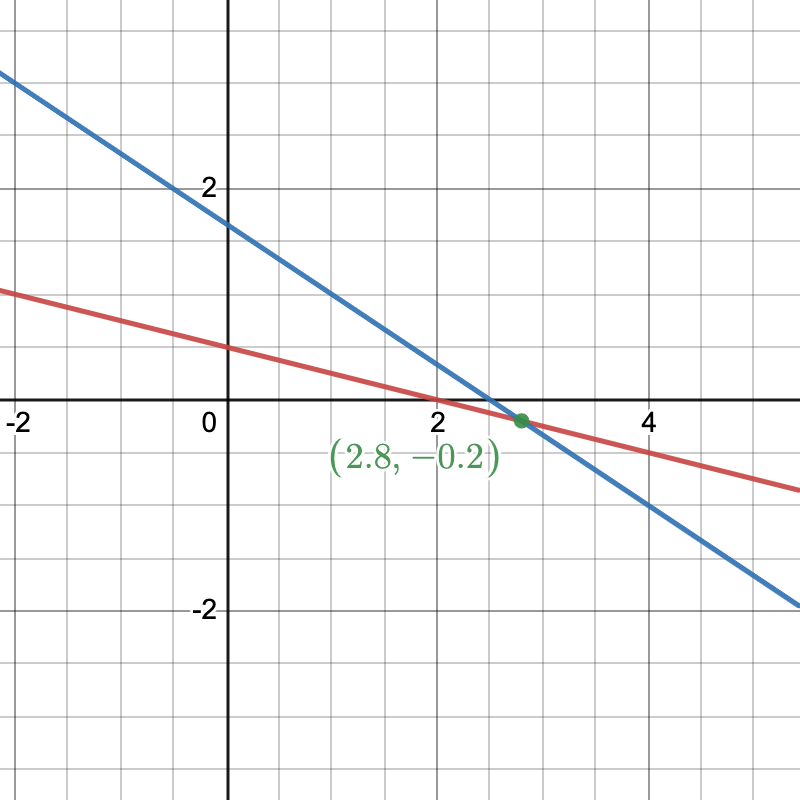
\includegraphics[width=7cm]{system-of-eqs.png}
  \centering
  \caption{Graph of a system of equations}
\end{figure}

We can see that there exists a solution where $x=2.8$ and $y = -0.2$. Very cool. Let's try a different example now, where we take the previous system and add a new, third equation onto it. 

\begin{example}
  \[
    \begin{cases}
      x + 4y = 2\\
      2x + 3y = 5\\
      2x + 3y = 4
    \end{cases}
  \]
\end{example}

\begin{figure}[H]
  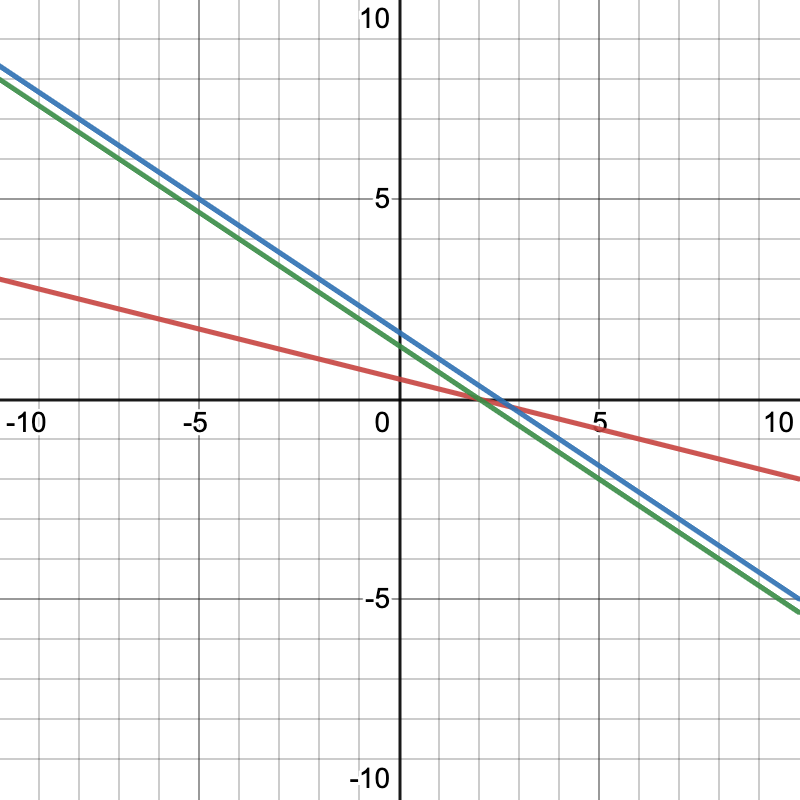
\includegraphics[width=7cm]{system-of-eqs(2).png}
  \centering
  \caption{Graph of a system of equations}
\end{figure}

Uh-oh. Now there's a problem. We can't find a common point of intersection between the three equations. This means that there isn't a single value of $x$ and $y$ that satisfies all three equations in the example. A situation like this is known as the system having \textbf{no solutions}.

Now, as I'm editing this book about three weeks after I first wrote this chapter, I'm starting to realize that I really don't want to open up desmos to create another visual example. We'll instead describe a very simple situation where a system will have an infinite number of solutions and call it a day. 

Consider the following system of two equations.

\begin{example}
  \[
    \begin{cases}
      x = y\\
      x = y
    \end{cases}
  \]
\end{example}

You'll notice (quite quickly, I'd hope) that the following system has two equivalent equations. What does that mean?

Well, if you try graphing the two equations, you'll notice that you'd end up drawing two lines right over each other. Thus, if you select any point within one equation, that point will also belong to the other equation. This means that there are an infinite number of points of intersection within this system, otherwise known as the system having \textbf{infinite solutions}.

Note that two equations don't necessarily have to be the same in order for them to have an infinite number of solutions! This may be true in the two-dimensional case, but it quickly falls apart in three-dimensions. Consider the case where you draw two different, intersecting planes in three dimensions. When you intersect two planes, will you always end up with one point of intersection? 

The answer is a resounding no. If you're curious why, you are encouraged to take a piece of paper and try folding it by half. Now, imagining each folded section of your paper as a separate plane, you'll note that the intersection between your two planes will always be a singular line no matter how you fold your paper. A line contains an infinite number of points, so we see that two intersecting planes will always have an infinite number of solutions.

As a matter of fact, a three variable system will always need at least three equations in order for it to have a unique solution. This is in fact true for any n-variable system of equations.  

In any case, the geometric method of solving systems of equations is by far the most straightforward and easy to understand. But as hinted before, the geometry of all this falls apart as soon as we use more than three variables. Here is where we decide to pull out the big guns: algebra. 

\subsection{Solving Through Elimination}

Recall that an equation is a statement asserting the \textbf{equality} of two equations. Thus our new method will very obviously have to take advantage of one of the properties of equality. Consider the following property. 

\begin{center}
  Given a, b, and c, if $a = b$, then $a + c = b + c$. If $c = d$, then $a + c = b + d$. 
\end{center}

We can apply this to our system of equations. Let's take a look at the system below. 

\[
  \begin{cases}
    x + 4y = 2\\
    2x + 3y = 5
  \end{cases}
\]

Let $a = 2x + 3y$, and $b = 5$. Then $c = x + 4y$ and $d = 2$. Then, our $a + c = b + d$ would be 

\begin{align*}
  3x + 7y = 7
\end{align*}

This is not very useful for our purpose. But what if we look at $a - c = b - d$?

\begin{align*}
  x - y = 3
\end{align*}

We can apply the process one more time to look at $a - 2c = b - 2d$. 

\begin{align*}
  - 5y = 1
\end{align*}

Then, with a little bit of algebraic manipulation, we see that $y = -\frac{1}{5}$. Substituting this value into $x + 4y = 2$, we see that $x - \frac{4}{5} = 2$ and $x = 2 + \frac{4}{5} = 2.8$. 

\textbf{tl;dr} So, going back to our initial system, we essentially took the first equation and subtracted it twice from the second equation in order to \textbf{eliminate} the $x$ variable. Of course, this process can be used to eliminate any variable(s) from an equation in a system. 

Let's now take a look at the system of equations that didn't have a solution from before.

\[
  \begin{cases}
    x + 4y = 2\\
    2x + 3y = 5\\
    2x + 3y = 4
  \end{cases}
\]

By subtracting the second equation from the third, we get:

\[
  \begin{cases}
    x + 4y = 2\\
    2x + 3y = 5\\
    0 = 1
  \end{cases}
\]

Now it's very evident that 0 does not equal 4. This means that there is an \textbf{inconsistency} in the system. When this happens, a solution cannot exist. Let's take a look at the modified version of this same problem.

\[
  \begin{cases}
    x + 4y = 2\\
    2x + 3y = 5\\
    2x + 3y = 5
  \end{cases}
\]

Then, again subtracting the second equation from the third equation: 

\[
  \begin{cases}
    x + 4y = 2\\
    2x + 3y = 5\\
    0 = 0
  \end{cases}
\]

This time we got $0=0$. This statement is true regardless of the values for $x$ and $y$. Thus, there are infinitely many solutions to this system of equations. 

\subsection{Word Problems}

In this subsection, we won't go over the strict strategy of analyzing word problems and solving them. I'll assume that you already know this, and will instead use an example from Eisner \cite{eisner:1994} to demonstrate the use case of system of equations.

Let's say say Steve held 100\% of stocks in a company at \$5000. The company decides to issue new stocks to Dave so that Dave would then own 5\% of the company. How much money would Dave's stocks be worth?

First we find the value for the new total value of outstanding stock.

\begin{align*}
  S = 5000 + x
\end{align*}

Where $S$ is the value of the outstanding stock, and $x$ is the stock issued to Dave. We also know that Dave's stock is worth 5\%. 

\begin{align*}
  x = 0.05S
\end{align*}

We now have a system of equations.

\[
  \begin{cases}
    S = 5000 + x\\
    x = 0.05S\\
  \end{cases}
\]

Rearranging the equations, we get the following.

\[
  \begin{cases}
    S - x = 5000\\
    -0.05S + x = 0\\
  \end{cases}
\]

Using our process of elimination, we simply add the bottom equation to the top to isolate $S$. 

\[
  \begin{cases}
    0.95S = 5000\\
    -0.05S + x = 0\\
  \end{cases}
\]

Then, $S = 5000 * \frac{1}{0.95} \approx 5263.16$, so Dave was awarded \$263.16 in total.  

\subsection{Problems}

For the next three problems, solve the given system of equations by graphing (you may use desmos). Indicate whether or not the system has solutions, no solutions, or infinite solutions.

\begin{exercise} Find the solution to the following system, if there are any.
  \[
    \begin{cases}
      2x + 3y = 10\\
      x + x + y = 0\\
      x + y = 2.5
    \end{cases}
  \]
\end{exercise}

\begin{exercise} Find the solution to the following system, if there are any.
  \[
    \begin{cases}
      x + 10y = 10\\
      x + x + y = 0\\
      x + y = 5
    \end{cases}
  \]
\end{exercise}

\begin{exercise} Find the solution to the following system, if there are any.
  \[
    \begin{cases}
      2x + 2y = 10\\
      x + y = 5
    \end{cases}
  \]
\end{exercise}

The next five problems will be difficult to solve using graphs. Good luck! Do not use a calculator.

\begin{exercise} Explain why the following system will have an infinite number of solutions.
  \[
    \begin{cases}
      2x + 2y + z = 10\\
      x + y + z = 5
    \end{cases}
  \]
\end{exercise}

\begin{exercise} Solve the following system of equations.
  \[
    \begin{cases}
      2x + 2y + z = 10\\
      x + y + z = 5\\
      y = 2
    \end{cases}
  \]
\end{exercise}

\begin{exercise} Explain why the following system will have no solutions.
  \[
    \begin{cases}
      2x + 2y + 2z = 15\\
      x + y + z = 5\\
    \end{cases}
  \]
\end{exercise}

\begin{exercise} Find the solution to the following system, if there are any.
  \[
    \begin{cases}
      x - 3y + z = 2\\
      3 x - 4 y + z = 0\\
      2 y - z = 1
    \end{cases}
  \]
\end{exercise}

\begin{exercise} Find the solution to the following system, if there are any.
  \[
    \begin{cases}
      2x + 2y + 3z = 15\\
      x + 2y + 2z = 2\\
      x + y + z = 5\\
      x + z = 12
    \end{cases}  
  \]
\end{exercise}

You may use a calculator to assist yourself in the following problem.

\begin{exercise}
  Steve sold 11 books and 13 pencils for 115 dollars total. If the books cost 10 dollars each, then how much do the pencils cost?
\end{exercise}

\section{Polynomial Arithmetic}

Polynomial expressions are undoubtedly one of the most powerful ways of using mathematics. For something so simple, so many of our problems in life or science can be modelled with it! It is probably one of our best ways to approximate the behavior of something we are trying to analyze. In this section, we won't spend time going over what a polynomial is. I will assume that you already know what they look like. They are not too difficult to figure out, so finding an online resource on what polynomials are should be sufficient otherwise. 

The central concern in this section regards situations where we have to consider the relationship of two different polynomial functions together. That is, how do we perform arithmetic between polynomials?

Thankfully, this is a solved problem. It turns out that polynomials behave very, very nicely under basic arithmetic operations. That is, when we add and multiply polynomials together, we'll always get a polynomial back. This isn't necessarily the case for division, but we won't be using a lot of that to begin with, so it's cool!

\subsection{Polynomial Addition}

Before anything else, let's go over the most basic way of classifying polynomials. This will be somewhat important to know!

Recall that the \textit{degree} of a polynomial refers to the highest power a term has in a given polynomial.

\[
  x^3 + x^2 + x + 1 = 0
\]

So, the degree of the above polynomial equation is 3. Now we can move on.

Also recall that variables of different powers cannot be added together. Consider the following polynomial of degree 4.

\[
  x^2 + x^4
\]

There is no way to simplify the above expression further. That is, there is no way of being able to add $x^2$ and $x^4$ together. Similarly, if the base (that is, the variables) of each term is different, we cannot add two terms together despite them having the same power. Let's take a look.

\[
  x^2 + y^2
\]

Again the above expression has no simplifications that could be applied to it. So given two polynomial expressions, how do we add the two together? It's simple, we \textbf{group like terms together}. Let's try adding the following two expressions. 

\begin{align*}
  x^2 + 2x + 1\\
  x^3 + 3x^2 + x + 4
\end{align*}

Now, we add them.

\[
  (x^2 + 2x + 1) + (x^3 + 3x^2 + x + 4)
\]

Now that we have the expression in this form, we simply have to group them term-by-term to simplify. 

\[
  (x^3) + (x^2 + 3x^2) + (2x + x) + (1 + 4)
\]

We add like terms together, and the simplification is complete.

\[
  x^3 + 4x^2 + 3x + 5
\]

What of polynomial \textit{equations}, then? We'll briefly go over the process of adding two equations together. It is not so different from what we did in the previous section with adding two linear equations together. 

\begin{align*}
  x^2 + 2x + 1 = 10\\
  x^3 + 3x^2 + x + 4 = 12
\end{align*}

Here we have the expressions from above turned into equations. When we add two polynomial equations, we simply add both sides of the equal signs together. 

\[
  (x^2 + 2x + 1) + (x^3 + 3x^2 + x + 4) = 10 + 12
\]

Then, everything simplifies like before.

\[
  x^3 + 4x^2 + 3x + 5 = 22
\]

And thus we have covered addition.

\subsection{Polynomial Substraction}

Subtraction works much in the same way as polynomial addition. Instead of adding, we just subtract! We'll take the two equations from before and try subtracting them from one another.

\begin{align*}
  x^2 + 2x + 1 = 10\\
  x^3 + 3x^2 + x + 4 = 12
\end{align*}

The process is identical from here on out. 

\begin{example}
\begin{align*}
  (x^2 + 2x + 1) - (x^3 + 3x^2 + x + 4) &= 10 - 12\\
  (-x^3) + (x^2 - 3x^2) + (2x - x) + (1 - 4) &= -2\\
  -x^3 - 2x^2 + x - 3 &= -2\\
\end{align*}
\end{example}

\subsection{Polynomial Multiplication}

Polynomial multiplication is a little bit more difficult than normal multiplication. The best way to go about this is to realize that multiplication is distributive over addition. That is, given real numbers $a, b, c$, we can do the following.

\[
  a(b + c) = ab + ac
\]

Polynomial multiplication works a lot like this. Except that we're multiplying two expressions with multiple terms together. Let's consider the case with real numbers $a, b, c, d$.

\begin{align*}
  (a + b)(c + d) &= (a + b)c + (a + b)d\\
  &= ac + bc + ad + bd
\end{align*}

As you saw above, you simply treat $(a + b)$ as a single element and proceed as before. Hopefully this isn't too difficult to think about. Let's try applying this to polynomial expressions.

\begin{example}
\begin{align*}
  (x + 2)(x^2 + x + 1) &= (x + 2)x^2 + (x+2)x + (x+2)1\\
  &= (x^3 + 2x^2) + (x^2 + 2x) + (x+2)\\
  &= x^3 + 3x^2 + 3x + 2
\end{align*}
\end{example}

Not too bad, right? In the end you're just breaking down the problem into easier subproblems and tackling them one at a time. 

\subsection{Polynomial Factoring}

Why is factoring polynomials important? Well, consider that you're trying to find the roots of a polynomial. A root of a polynomial is a value $x_0$ where, given a polynomial function $p(x)$, $p(x_0) = 0$. If you were to be told to find the roots of the polynomial $p(x) = x^2 - 24x + 144$, it wouldn't immediately be obvious how one might find them. But if the polynomial were to be given in the following form,

\[
  p(x) = x^2 -24x + 144 = (x - 12)(x - 12) = 0
\]

It's immediately obvious to us that the root of our polynomial (of which there is only one) is 12. 

But this does beg the question. Why in the world are we looking for solutions to polynomials that equal to 0? Why not anything else? Surely it's far more useful to compute solutions to polynomial functions when they equal any other constant! Well, consider the following example. Let's say you have a polynomial function $p(x)$ that models the behavior of, say, the value of a particular stock. Given that $x$ is a variable on time, you're looking for when $p(x) = 148$. But then consider this.

\begin{align*}
  p(x) &= 148\\
  p(x) - 148 &= 0
\end{align*}

The function $p(x) - 148$ is still a polynomial! Moreover, we've reduced the problem into one where we only have to find the roots of this new polynomial. All we have to do from this point is to factor it!

You can think of polynomial factoring as the polynomial version of division. In competitive mathematics, it's often required for you to know how to factor polynomial equations of up to three or four degrees. We'll just cover the case of quadratics (polynomials of degree two) here.

\subsubsection{Difference of Squares}

Really, the difference of squares technique is just a special case of factoring a quadratic polynomial. The reason why it's called such is because you're subtracting two square numbers from each other. Behold. Given two numbers a and b...

\[
  a^2 - b^2 = (a + b)(a - b)
\]

Feel free to multiply out the right hand side of the equation to verify that this is true. In any case, this relation obviously holds true for polynomials as well. Here is an example.

\begin{example}
\[
  x^2 - 4 = (x + 2)(x - 2)
\]
\end{example}

At this point, you might be wondering if this is only possible for quadratics. Not so! Let's think about this for a second.

\[
  x^4 - 4
\]

We simply realize here that $x^4$ is, in fact, a square of a number--- $x^2$! Thus we can use the difference of squares to nicely factor our polynomial.

\begin{example}
\[
  x^4 - 4 = (x^2 + 2)(x^2 - 2)
\]
\end{example}

We can note here that a number or a variable is a square so long as its power is divisible by 2. Here's a slightly bigger, a little bit more interesting example of the difference of squares in action.

\begin{example}
  \begin{align*}
    x^8 - 256 &= (x^4 + 16)(x^4 - 16)\\
    &= (x^4 + 16)(x^2 + 4)(x^2 - 4)\\
    &= (x^4 + 16)(x^2 + 4)(x + 2)(x - 2)
  \end{align*}
\end{example}

Pretty neat, huh? Now that's try completing the square instead of taking the difference of them.

\subsubsection{Completing the Square and Stuff}

Completing the square is exactly like multiplying two polynomials together, but in reverse. Consider a previous example.

\begin{align*}
  (a + b)(c + d) &= (a + b)c + (a + b)d\\
  &= ac + bc + ad + bd
\end{align*}

Changing this to a formula for quadratics, we get this. You might recognize this as the FOIL method.

\begin{align*}
  (x + a)(x + b) &= (x + a)x + (x + a)b\\
  &= x^2 + ax + bx + ab\\
  &= x^2 + (a + b)x + ab
\end{align*}

We could also have a case where we're multiplying the two same terms together. In this case computation becomes easier.

\begin{align*}
  (x + a)^2 &= (x + a)(x + a) \\ 
  &= (x + a)x + (x + a)a\\
  &= x^2 + ax + ax + a^2\\
  &= x^2 + 2ax + a^2
\end{align*}

Reversing the process, then, is simple. Let's try it out on a few examples.

\begin{example}
  First we factor $x^2 + 10x + 25$. Note $2 * 5 = 10$ and $5^2 = 10$. 
  \begin{align*}
    x^2 + 10x + 25 &= (x + 5)^2
  \end{align*}
\end{example}

\begin{example}
  Given $x^2 - 4x + 4$. Note $-2 -2 = -4$, and $(-2) * (-2) = 4$. 
  \begin{align*}
    x^2 -4x +4 &= (x - 2)^2
  \end{align*}
\end{example}

In cases like these the patterns are fairly simple to identify. Now let's try identifying the factorizations for polynomials that are a bit dirtier than this.

\begin{example}
  First we factor $x^2 + 7x + 10$. Note $2 + 5 = 7$ and $2 * 5 = 10$. 
  \begin{align*}
    x^2 + 7x + 10 &= (x + 2)(x + 5)
  \end{align*}
\end{example}

\begin{example}
  Given $x^2 + 3x - 10$. Note $-2 + 5 = 3$, and $-2 * 5 = -10$. 
  \begin{align*}
    x^2 + 3x - 10 &= (x - 2)(x + 5)
  \end{align*}
\end{example}

Unfortunately, the only way for you to ,be able to be able to do this quickly is to do many of them to build intuition. But the process isn't so bad! You'll quickly get used to it.

\subsubsection{Quadratic Formula}

But what if you have a polynomial that's crazy, such as $x^2 - x - 1$? How in the world do you find a root for a quadratic like this? Fortunately, quadratics are very cool in that we have a formula for finding their roots! This is the famous binomial formula.

Given a polynomial $ax^2 + bx + c = 0$, one can compute the roots of this polynomial with the following.

\begin{align*}
  x = \frac{-b \pm \sqrt{b^2 - 4ac}}{2a}
\end{align*}

Using this formula, we find that the roots of our polynomial is $\frac{1 + \sqrt{5}}{2}$ and $\frac{1 - \sqrt{5}}{2}$. This is the famous golden ratio. It is not a mistake that it appears as a root of our polynomial. We will not go over why in this text, though. 

It seems almost unbelievable that we have such a simple formula for computing the roots of any given polynomial. Indeed, this is not a normal occurence at all. We have formulas for finding roots of degree 1, 2, 3 and 4 polynomials. However, mathematicians Paolo Ruffini and Niels Henrik Abel proved that no such a formula exists for polynomials of degree 5 or higher.

The derivation of this formula is actually pretty simple. We'll be using a shorter, less intuitive version of it just for the sake of saving space. The derivation is provided courtesy of Larry Hoehn \cite{hoehn:1975}.

Provided $ax^2 + bx + c = 0$, we start off by multiplying both sides of the polynomial by $4a$. So now we have

\[
  4a^2x^2 + 4abx + 4ac = 0
\]

We rearrange.

\[
  4a^2x^2 + 4abx = -4ac
\]

Add $b^2$ to both sides.

\[
  4a^2x^2 + 4abx + b^2 = b^2-4ac
\]

Notice the left side of the equation can be factored.

\[
  (2ax + b)^2 = b^2-4ac
\]

We can take the square root of both sides.

\[
  2ax + b = \pm\sqrt{b^2-4ac}
\]

Now it's just a simple matter of isolating $x$ on the left side.

\begin{align*}
  x = \frac{-b \pm \sqrt{b^2 - 4ac}}{2a}
\end{align*}

Normally, it takes too much work to compute the roots of a quadratic using a formula as compared to factoring using intuition to find the roots. But when your intuition fails, the formula can come in to save the day.

\subsection{Problems}

Writing this was an entire journey. Thankfully, writing these problems will be incredibly easy in comparison.

\begin{exercise}
  Add $x^2 + x - 10$ and $10x^2 + 3x + 10$.
\end{exercise}

\begin{exercise}
  Add $x^5 + x^4 + x^3 + 1$ and $3x^4 + x^2 + 10$.
\end{exercise}

\begin{exercise}
  Subtract $5x^3 - x^2 + 5x + 10$ from $x^3 + x^2 - 3x + 10$.
\end{exercise}

\begin{exercise}
  Multiply $x + 1$ with $x^2 + 2x + 5$.
\end{exercise}

\begin{exercise}
  Multiply $x^2 + x + 1$ with $2x^3 + 2x + 5$.
\end{exercise}

\begin{exercise}
  Factor $x^2 + 6x + 9$ into its lowest terms.
\end{exercise}

\begin{exercise}
  Factor $x^8 - 49$ into its lowest terms.
\end{exercise}

\begin{exercise}
  Factor $x^2 - 10x + 24$ into its lowest terms.
\end{exercise}

\begin{exercise}
  Factor $x^2 + 11x + 30$ into its lowest terms.
\end{exercise}

\begin{exercise}
  Factor $x^2 + 3x + 3$ into its lowest terms. Use the quadratic formula. 
\end{exercise}

\begin{exercise}
  Factor $x^2 + 2x + 11$ into its lowest terms. Use the quadratic formula. 
\end{exercise}

\begin{exercise}
  Use the quadratic formula to find the roots of $3x^2 + 2x + 10$.
\end{exercise}

\section{Rational Exponents}

Rational exponents are expressions with fractions as exponents instead of natural numbers. The simplest example of this would be roots of a number. Let's take a look.

\begin{example}
  $\sqrt{4} = 4^{1/2} = 2$
\end{example}

\begin{example}
  $\sqrt[3]{27} = 27^{1/3} = (3 * 3 * 3)^{1/3} = 3$
\end{example}

Hopefully the concept of taking a root of a number is familiar to you. Rational exponents is a fairly intuitive extension of this idea. Given a number $x, a, b$, all of which are rational, 

\begin{align*}
  x^{a/b} = \sqrt[b]{x^a} = (\sqrt[b]{x})^a
\end{align*}

What does this mean? Let's step back for a second and think about roots again. To say $x^{1/3}$ means that there exists some number $s$ such that $s^3 = x$. Then, we can simply define $x^{2/3}$ to be a number $s$ such that $s^3 = x^2$. 

Let's take a look at a couple of examples.

\begin{example}
  $\sqrt[3]{27^2} = 27^{2/3} = (\sqrt[3]{27})^2 = 3^2 = 9$
\end{example}

\begin{example}
  
\end{example}

At this point you'll start to wonder how on earth people actually compute numbers like these. For example, how on earth are you supposed to know how to compute the square root of two? Or even worse, something like $2^{2/3}$? Here's how the computer does it.

From this point on, you can think of this as recreational mathematics. Even if you don't necessarily understand it, that's fine! Think of this like a very short 3-minute show that shows you how math typically works under the hood. 

We'll take a look at two methods. One that uses very basic mathematics to go ``searching'' for our desired number, and one method that makes use of exponential rules and logarithms to compute it. 

\subsection{Shifting $n$-th root algorithm}

Let's take a look at the problem one more time. Given $x, a, b$ all rational, we're trying to find some number $s$ such that $x^{a/b} = s$. 

We start off by trying to divide this problem into smaller subproblems that are easier to solve. First, we realize that taking the simple power of numbers--- such as $x^a$--- is actually very fast! It's just multiplication, which we are fairly good at. So we can ignore that for now.

The problem comes when we try to compute $x^{1/b}$, or the $b$-th root of $x$. Thankfully, the ancients have crafted a very nice method that's similar to long division in order to compute this number. 

The following algorithm is known as the \textbf{Shifting $n$-th root algorithm}. 

\subsection{Logarithmic Method for Computing Rational Exponents}

This is a method used by some computers and calculators to compute rational exponents!

\section{Exponentials and Logarithms}

Exponentials, logarithms, and trigonometry. This is a very special section of algebra (even though it technically isn't algebra at all), 

\subsection{Problems}

\section{Trigonometry}

\subsection{Problems}

\printbibliography

\end{document}
